
\begin{frame}[fragile,label=lostAdds]{lost adds (program)}
\begin{lstlisting}[language=myasm,style=smaller]
.global update_loop
update_loop:
    addl $1, the_value // the_value (global variable) += 1
    dec %rdi           // argument 1 -= 1
    jg update_loop     // if argument 1 >= 0 repeat
    ret
\end{lstlisting}
\hrule
\begin{lstlisting}[language=C++,style=smaller]
int the_value;
extern void *update_loop(void *);
int main(void) {
    the_value = 0;
    pthread_t A, B;
    pthread_create(&A, NULL, update_loop, (void*) 1000000);
    pthread_create(&B, NULL, update_loop, (void*) 1000000);
    pthread_join(A, NULL);
    pthread_join(B, NULL);
    // expected result: 1000000 + 1000000 = 2000000
    printf("the_value = %d\n", the_value);
}
\end{lstlisting}
\end{frame}

\begin{frame}[fragile,label=lostAddsResult]{lost adds (results)}
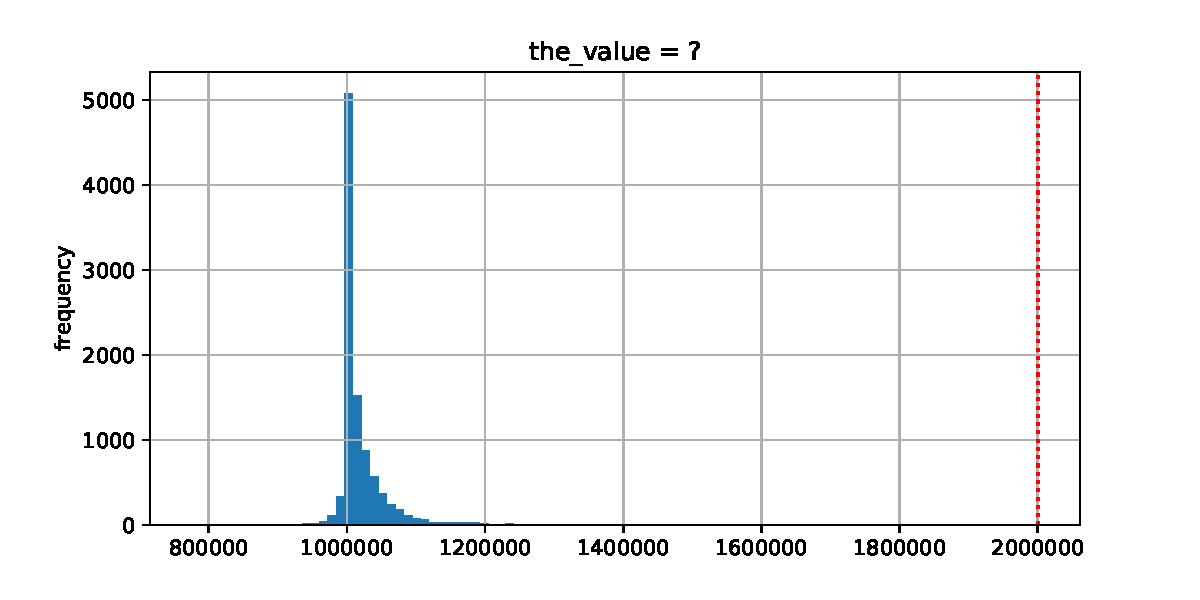
\includegraphics[width=1.1\textwidth]{../sync/parallel-add-histogram}
\end{frame}

\begin{frame}{but how?}
    \begin{itemize}
    \item probably not possible on single core
        \begin{itemize}
            \item exceptions can't occur in the middle of \texttt{add} instruction
        \end{itemize}
    \item \ldots but `add to memory' implemented with multiple steps
        \begin{itemize}
        \item still needs to load, add, store internally
        \item can be interleaved with what other cores do
        \end{itemize}
        \vspace{.5cm}
    \item<2-> {\small (and actually it's more complicated than that --- we'll talk later)}
    \end{itemize}
\end{frame}

